\section{Research \& development}
This department of AllSpark is involved in all the activities related to
improve and realize new products as research projects. This sector is
considered a relevant one in the organization business, in fact this sector
has the aim to bring innovation and distinguish our products among the
competitors.

An important feature of this area is the strong collaboration between
AllSpark and various foundation operating in the OpenSource community
environment.
These collaborations are based on active support of AllSpark during the
development of their project. The support AllSpark is offering id mainly
focused on patching and bugfixing, but can be expanded to founding or other
ways of collaboration.

\subsection{Search Sector}
The main aim of this process is to look for a research sector in which
instantiate a new r\&d project. Mainly is devolved to handle security
related sectors, due to the high risks and frequent changes always present
in this area.

The process involves an analysis of the newest studies on security issues
and menaces in IT systems, its results are useful for performing an
investigation about possible vulnerabilities in AllSparks products. Is
important to notice that other than check a single product is important to
consider the whole offer of AllSpark, looking for possible problems which
are not covered by the existing products but still in the scope of AllSpark
activity.

Image \ref{2img:sector} describes this process in its details.

\begin{figure}[!ht]
\begin{centering}
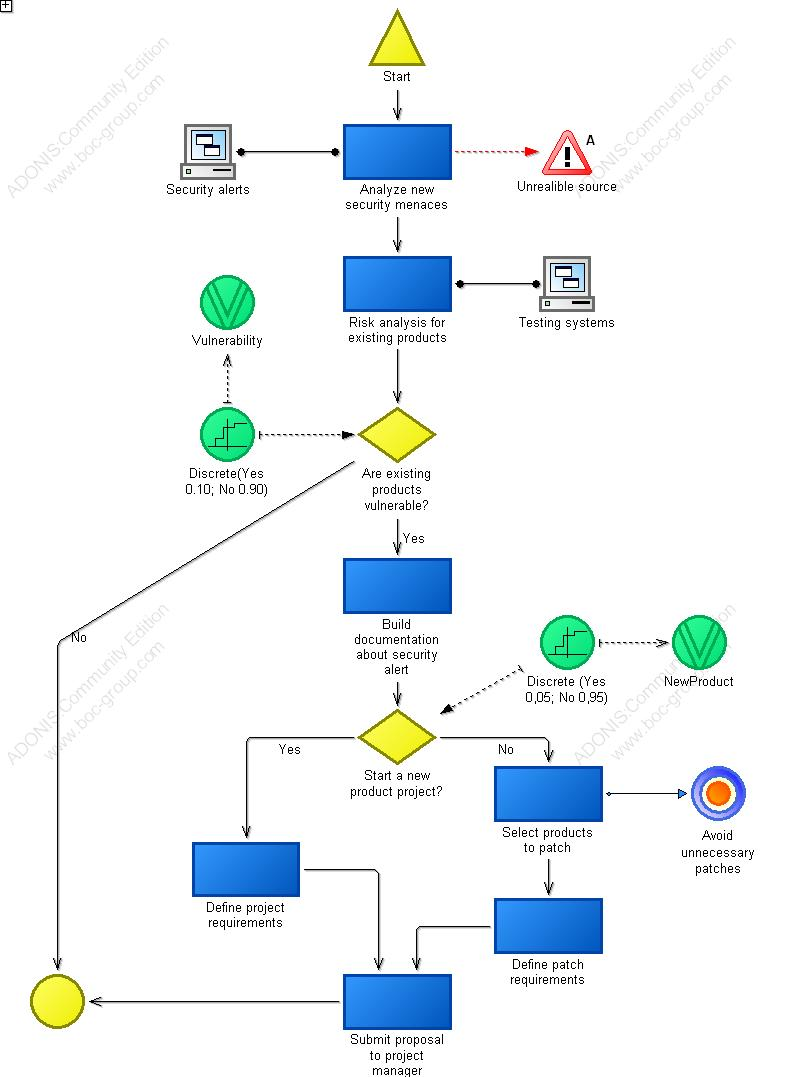
\includegraphics[scale=0.50]{assign2/adonis/imgs/sector.jpg}
\caption{Search sector AllSpark process}
\label{2img:sector}
\end{centering}
\end{figure}


\subsection{Search Updates}
In the IT environment trends and actual needs are often changing, is
therefore necessary to track these development in order to be prepared and
offer always updated products which can actually encounter costumer's
needs.

The aim of this process is to analyze the evolving market data and monitor
the trends in products usage. In this way AllSpark can retrieve a reliable
picture of the market trends.
The results of this analysis can be used to check whether there is the need
for developing a new product, or if is sufficient to add new features and
extensions to an existing one.

This process is depicted in image \ref{2img:search_upd}.

\begin{figure}[!ht]
\begin{centering}
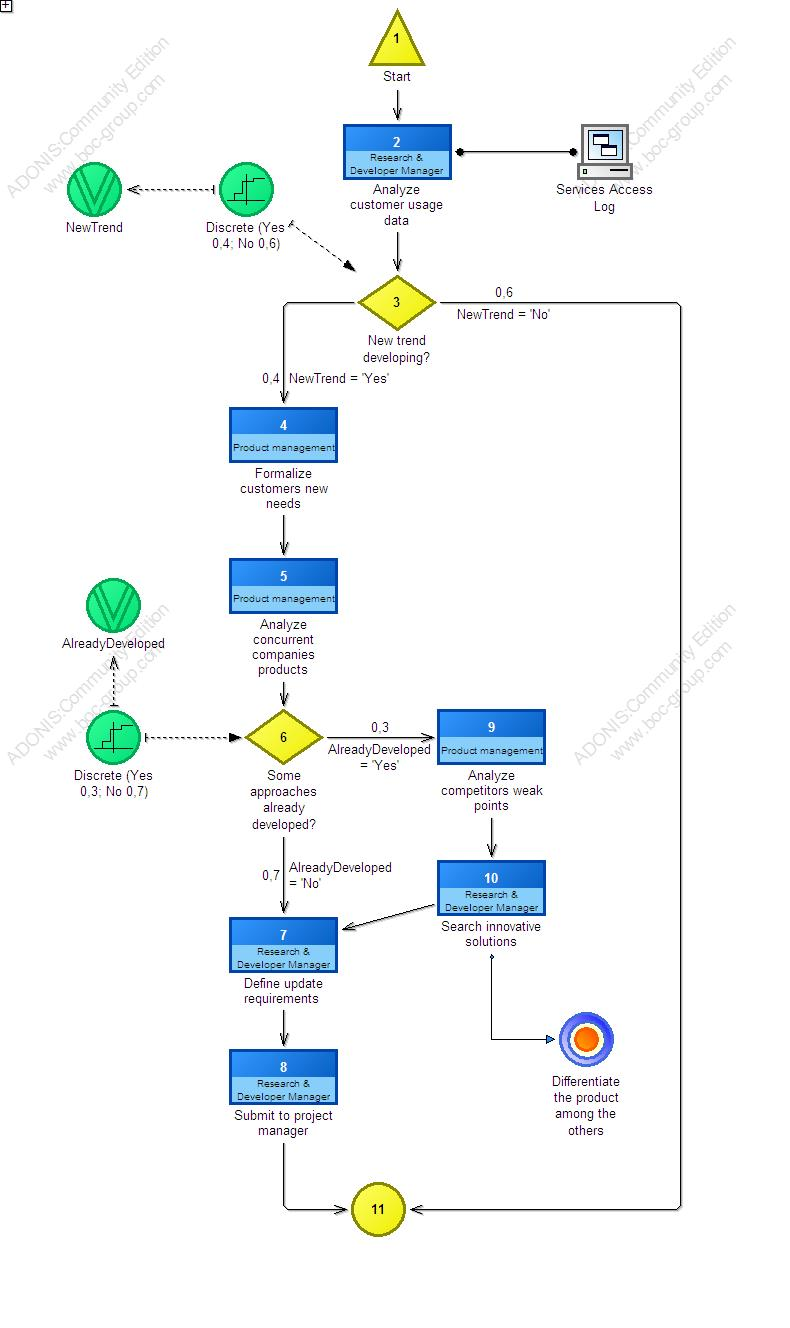
\includegraphics[scale=0.50]{assign2/adonis/imgs/search_upd.jpg}
\caption{Update searching process}
\label{2img:search_upd}
\end{centering}
\end{figure}

\subsection{Search bug}
This process describes how AllSpark handles with failures in its own
research project. In this process, in fact, developers are involved in
finding and fixing errors in existing projects.

In this process the main attention is focused on performing smart tests in
order to find and resolve the problems. One important thing is to notice
the difference between the two kinds of test which are going to be
performed.
In fact, after a first analysis of the code, is necessary to develop a
series of test cases which provides a wide coverage over the possible
different behaviour of the system. When the bug is located and a patch is
prepared, a sharper approach is needed, in order to test that particular
portion of the system. The process used in AllSpark to deal with bug
problems in research project is described in figure \ref{2img:search_bug}.

\begin{figure}[!ht]
\begin{centering}
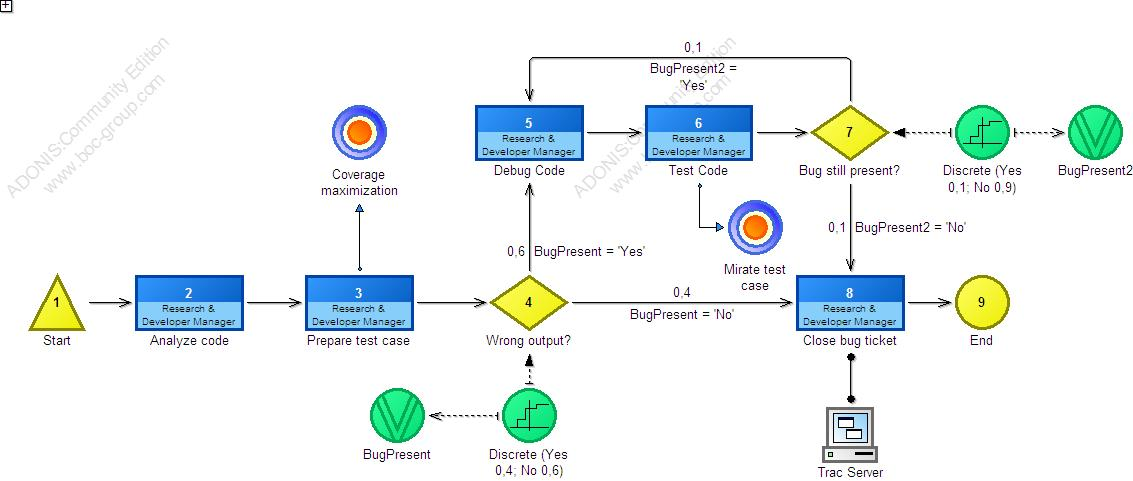
\includegraphics[scale=0.50, angle=90]{assign2/adonis/imgs/debug.jpg}
\caption{AllSparks debug process for Research project}
\label{2img:search_bug}
\end{centering}
\end{figure}

\subsection{Foundation Cooperation}
As said before, one of the aim of AllSpark is be engaged in an active
collaboration with the entities working in the OpenSource field. The
benefit of this collaboration is to be evaluated in an economic sense from
one side, and from a reputation point of view form the other.

For the foundations could be an opportunity to gain renown if AllSpark
products integrate their solutions. Apart from this the collaboration can
be based on financial founding or, as in the case of the research project,
on active collaboration on software developing.

This collaboration extends to bugfixing and patching the software, not to
strategic decisions on the direction of the development, this to preserve
the independence of the Foundation in its business.

The project of the patching activities for software not developed by
AllSpark, but by an OpenSource Foundation is described by figure
\ref{2img:found_coop}

\begin{figure}[!ht]
\begin{centering}
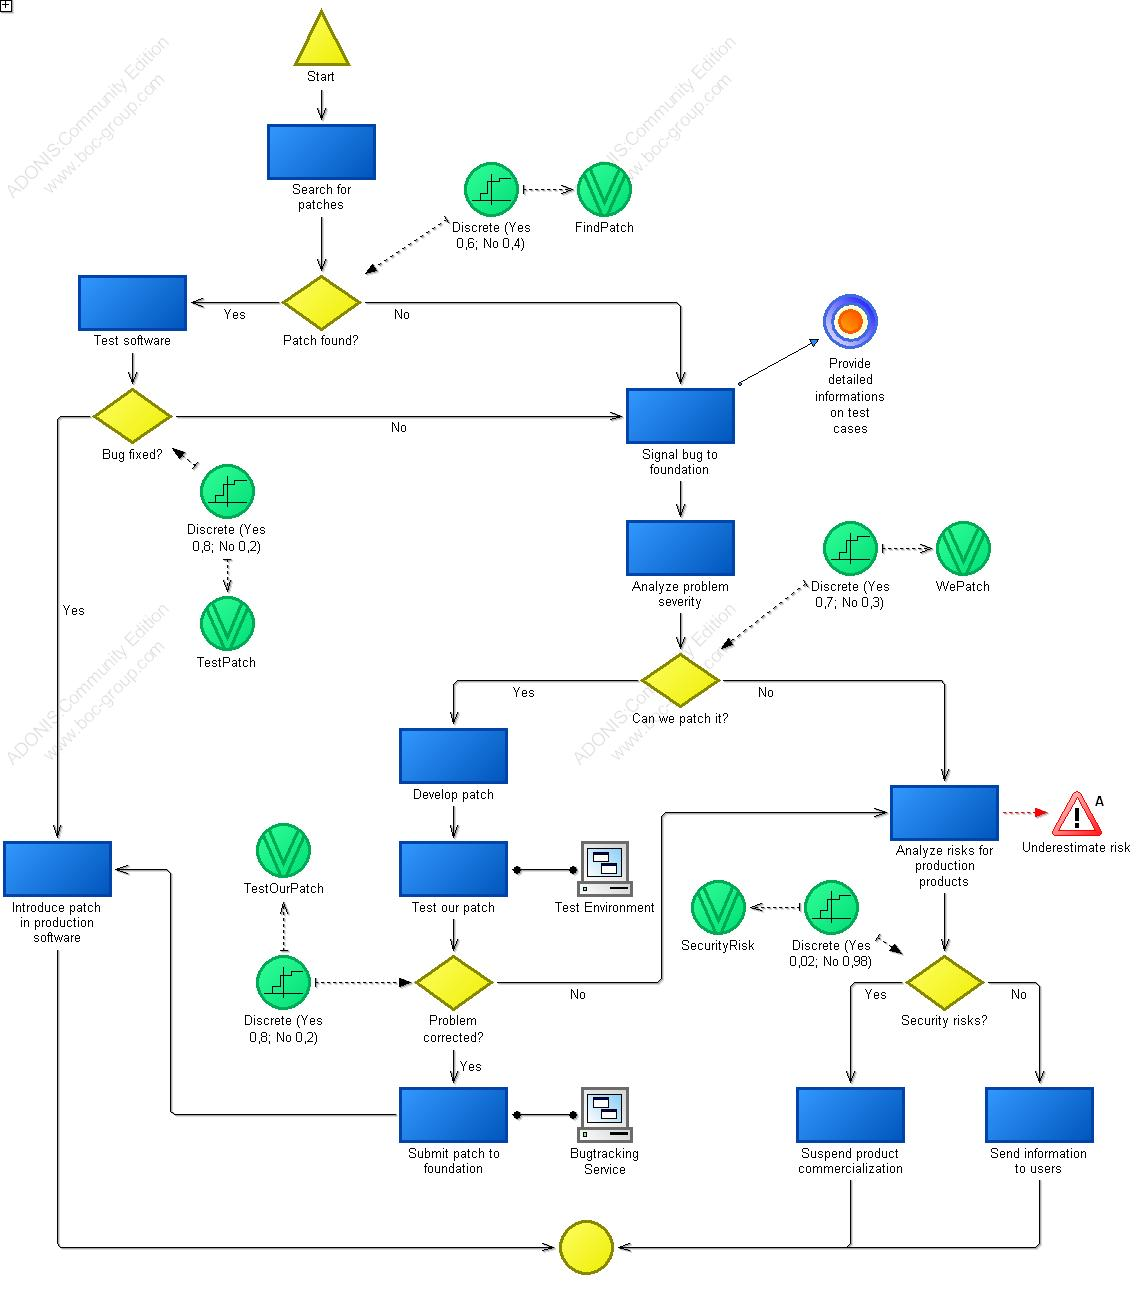
\includegraphics[scale=0.40]{assign2/adonis/imgs/coop.jpg}
\caption{Collaboration between AllSpark and OpenSource projects}
\label{2img:found_coop}
\end{centering}
\end{figure}

\subsection{Commercialization}
This process manages the procedure executed to evaluate if a research
project is ready to be actually converted in a effective product.
Is important to notice that this decision depends on on the market data and
on the need of the customer.

It can be the case that a project is not ready to be commercialized, or,
instead, the project is ready but the market and the customers don't yet
need this new product, at this moment.

If this is the case, is necessary to delay the commercialization of the
product waiting for a moment in which it can be more appreciated.
This process is described in figure \ref{2img:commerce}

\begin{figure}[!ht]
\begin{centering}
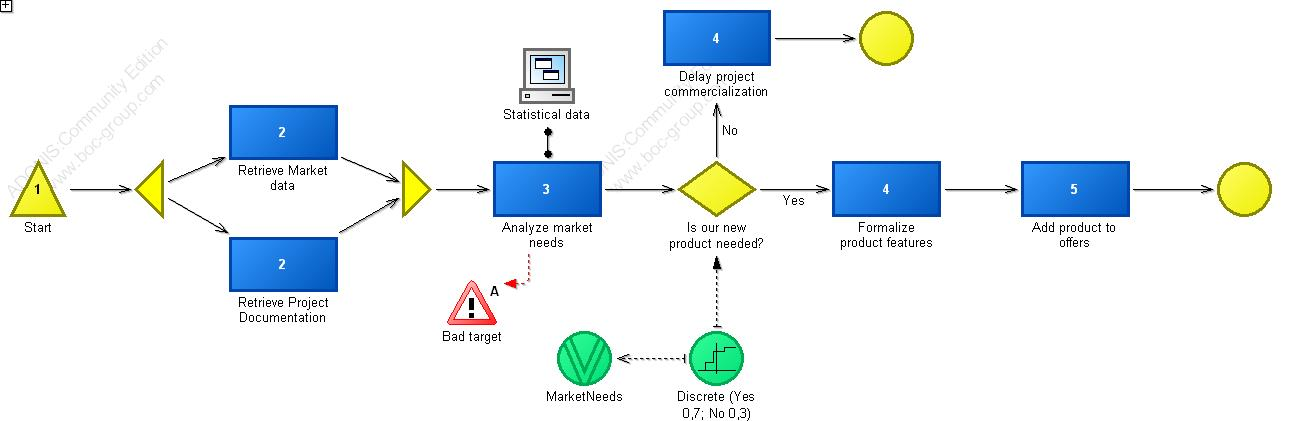
\includegraphics[scale=0.45,angle=90]{assign2/adonis/imgs/commercialize.jpg}
\caption{Commercialization of a research project}
\label{2img:commerce}
\end{centering}
\end{figure}



